\begin{frame}
	\frametitle{Markov chain}
	\begin{definition}
		A Markov chain is a stochastic process describing a sequence on some countable state space $S$ in which the probability of each event depends only on the state of previous event.
	\end{definition}
	\begin{definition}
		 Such a chain is uniquely defined by a stochastic transition matrix $\PP$ and a initial distribution $\mu$.
	\end{definition}
	\begin{figure}[!htb]
		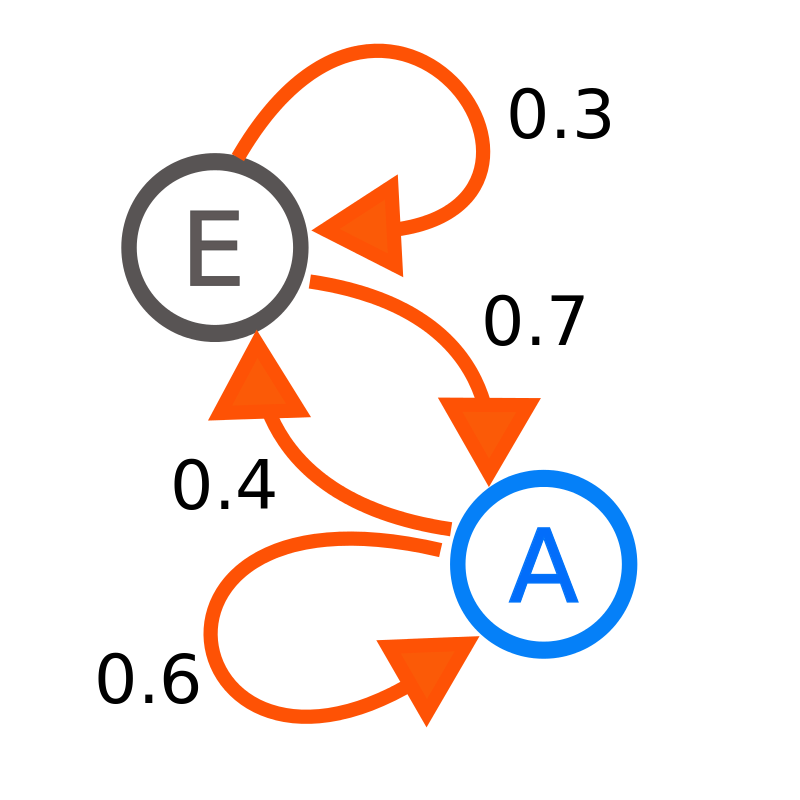
\includegraphics[scale=0.085]{img/Markov_diagram.png}
		\caption{A diagram representing a two-state Markov chain, source: wiki.}
	\end{figure}
\end{frame}

\begin{frame}
	\frametitle{Properties}
	\begin{definition}[Irreducibility]
		A Markov chain is irreducible if there is a possibility to reach every state from every state.
	\end{definition}

	\begin{definition}[Aperiodicity]
		A state is aperiodic if there is a possibility of coming back to it after each step. A Markov chain is aperiodic when every state is irreducible and a state is aperiodic.
	\end{definition}
	
\end{frame}

\begin{frame}
	\frametitle{Ergodic chains}
	\begin{definition}[Stationarity]
		A probability distribution $\bfpi = (\pi_1, \ldots, \pi_N)$ is called stationary if it satisfies
		\begin{equation*}
		\pi_j = \sum_{i \in S} \pi_i p_{ij},
		\end{equation*}
	\end{definition}
	\begin{definition}[Ergodicity]
		A Markov chain is ergodic when it is irreducible and aperiodic.
	\end{definition}
	\begin{theorem}
		Let $\left\{X_k\right\}$ be a ergodic Markov chain with a transition matrix $\PP$, then:
		\begin{equation*}
		\lim_{k \rightarrow \infty} p_{ij}(k) = \pi_j.
		\end{equation*}
	\end{theorem}
\end{frame}